\bivtask{Ein einfaches Antialiasing-Verfahren für Linien}{8}
%
Ergänzen Sie in der Datei \texttt{antial.cc} unter
\bivfolder{/home/bildgen/Aufgaben/anti-aliasing} die Funktion
\vspace{-\baselineskip}
\vspace{-.5em}
\begin{alltt}
   drawAntialiasedWideLine, 
\end{alltt}
\vspace{-.5em}
die geglättete Linien beliebiger Breite zeichnet.

\begin{center}
  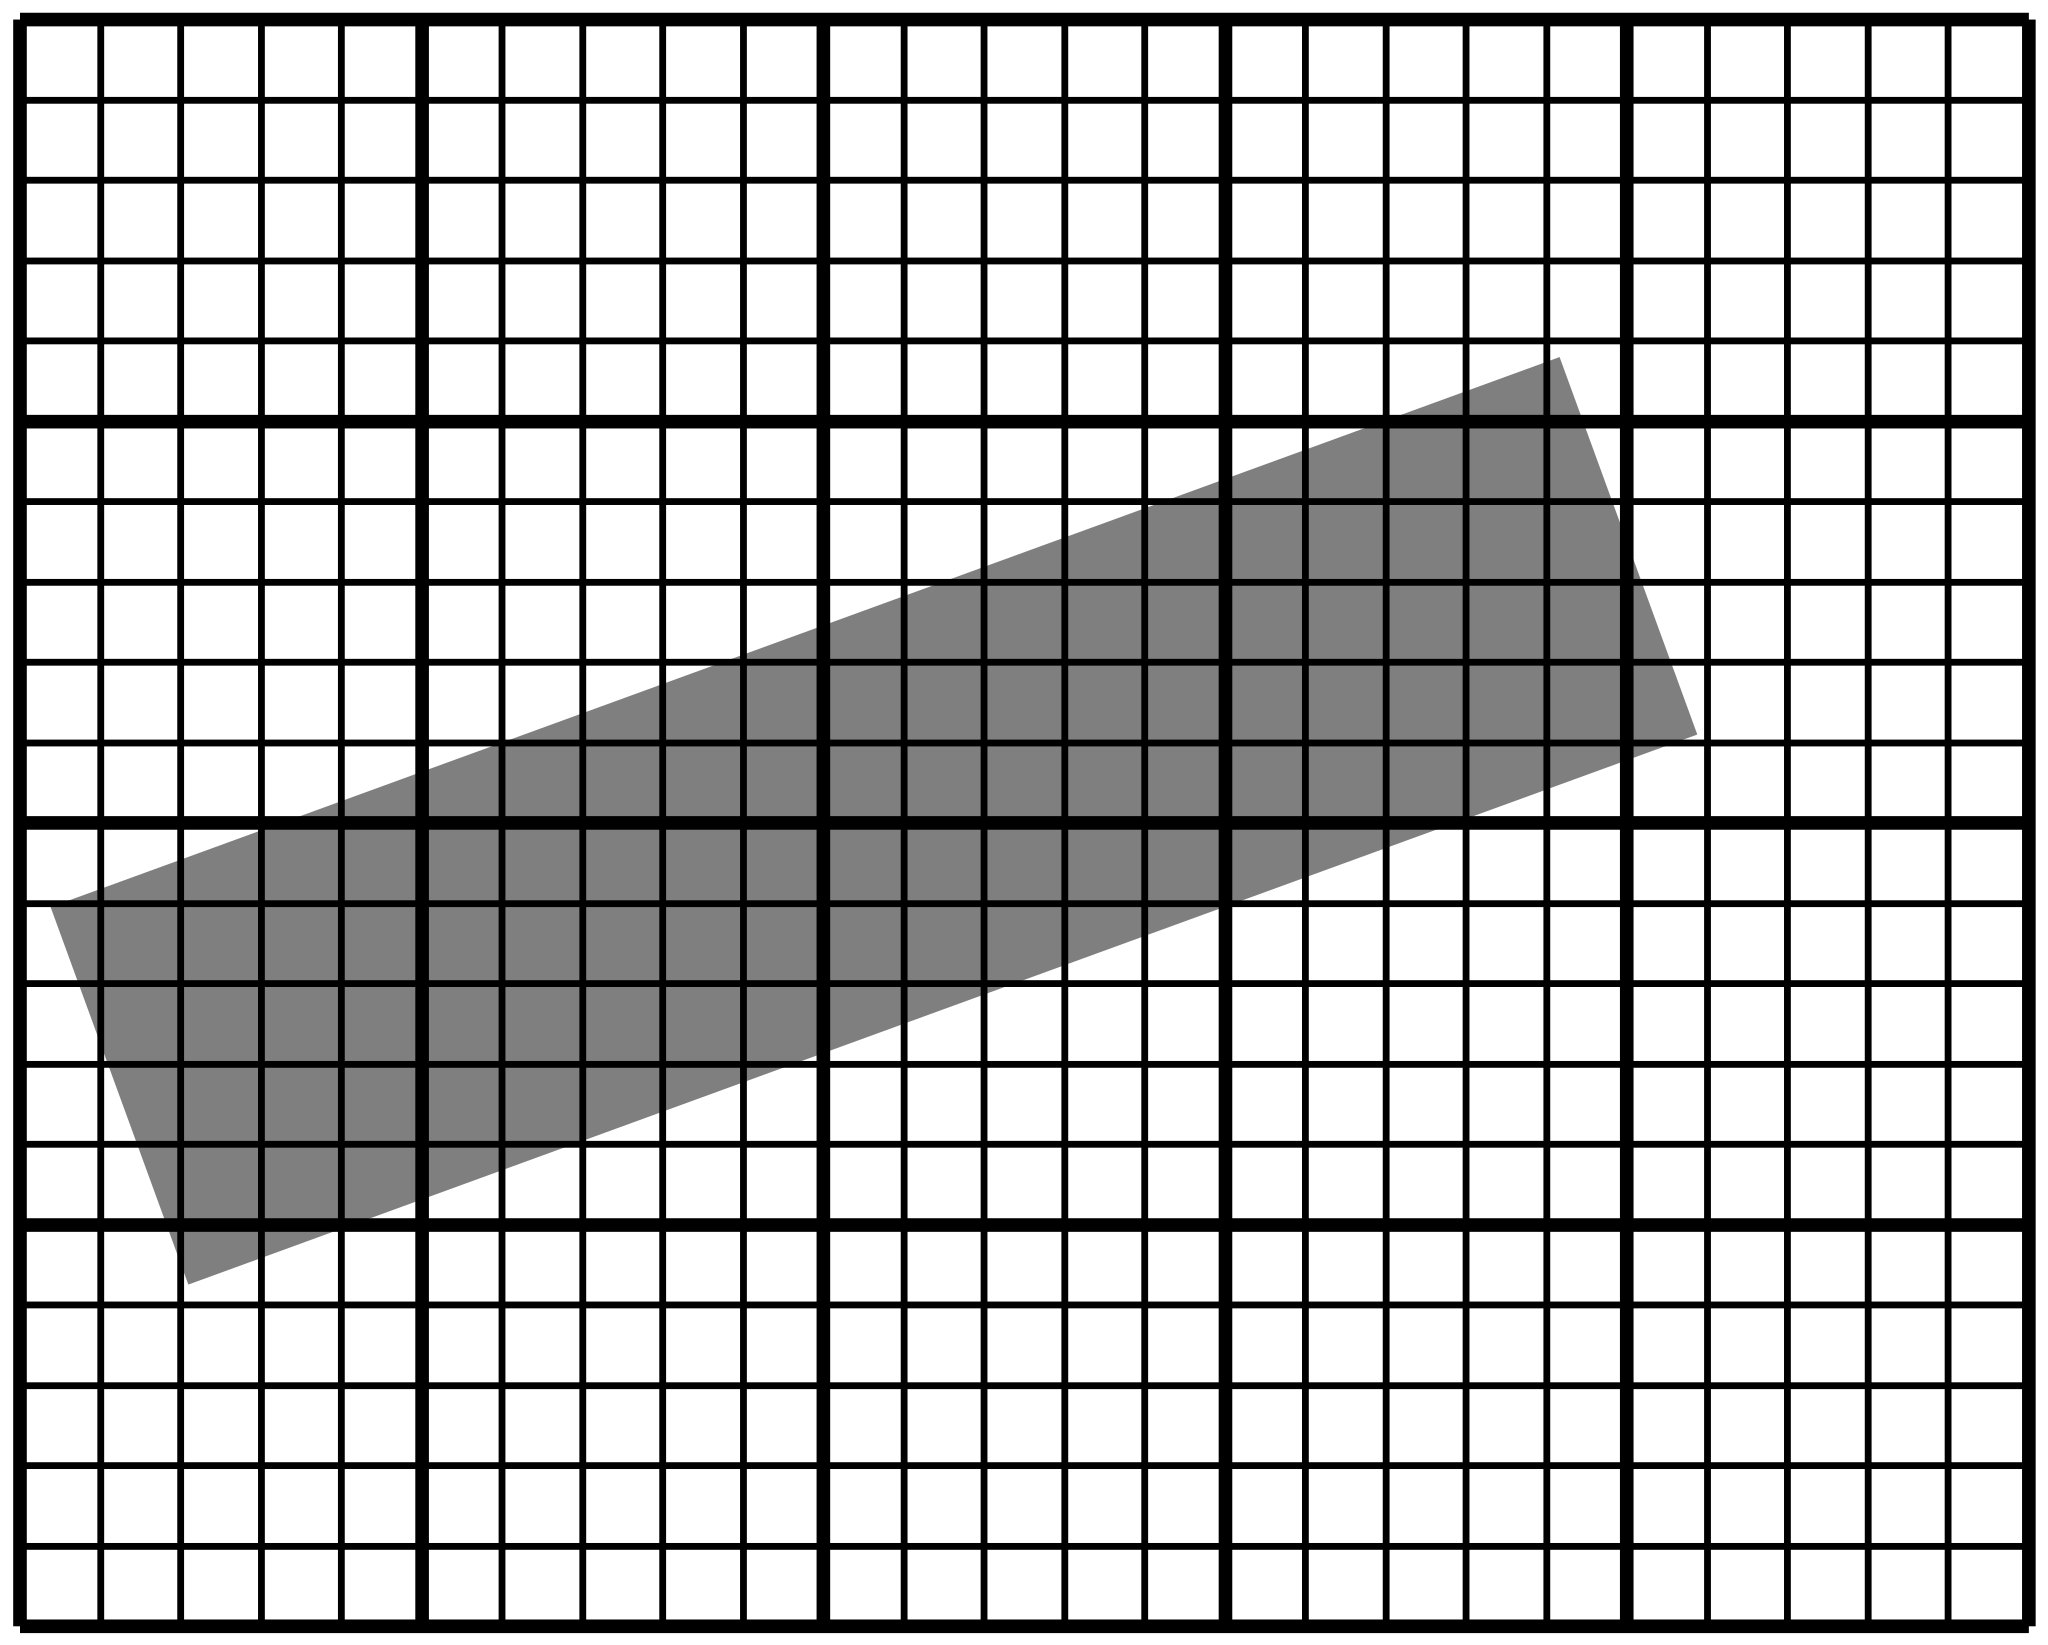
\includegraphics{antial1} \raisebox{4.5em}{→} %% Creator: Inkscape inkscape 0.91, www.inkscape.org
%% PDF/EPS/PS + LaTeX output extension by Johan Engelen, 2010
%% Accompanies image file 'antial2.pdf' (pdf, eps, ps)
%%
%% To include the image in your LaTeX document, write
%%   \input{<filename>.pdf_tex}
%%  instead of
%%   \includegraphics{<filename>.pdf}
%% To scale the image, write
%%   \def\svgwidth{<desired width>}
%%   \input{<filename>.pdf_tex}
%%  instead of
%%   \includegraphics[width=<desired width>]{<filename>.pdf}
%%
%% Images with a different path to the parent latex file can
%% be accessed with the `import' package (which may need to be
%% installed) using
%%   \usepackage{import}
%% in the preamble, and then including the image with
%%   \import{<path to file>}{<filename>.pdf_tex}
%% Alternatively, one can specify
%%   \graphicspath{{<path to file>/}}
%% 
%% For more information, please see info/svg-inkscape on CTAN:
%%   http://tug.ctan.org/tex-archive/info/svg-inkscape
%%
\begingroup%
  \makeatletter%
  \providecommand\color[2][]{%
    \errmessage{(Inkscape) Color is used for the text in Inkscape, but the package 'color.sty' is not loaded}%
    \renewcommand\color[2][]{}%
  }%
  \providecommand\transparent[1]{%
    \errmessage{(Inkscape) Transparency is used (non-zero) for the text in Inkscape, but the package 'transparent.sty' is not loaded}%
    \renewcommand\transparent[1]{}%
  }%
  \providecommand\rotatebox[2]{#2}%
  \ifx\svgwidth\undefined%
    \setlength{\unitlength}{141.63348784bp}%
    \ifx\svgscale\undefined%
      \relax%
    \else%
      \setlength{\unitlength}{\unitlength * \real{\svgscale}}%
    \fi%
  \else%
    \setlength{\unitlength}{\svgwidth}%
  \fi%
  \global\let\svgwidth\undefined%
  \global\let\svgscale\undefined%
  \makeatother%
  \begin{picture}(1,0.80117697)%
    \put(0,0){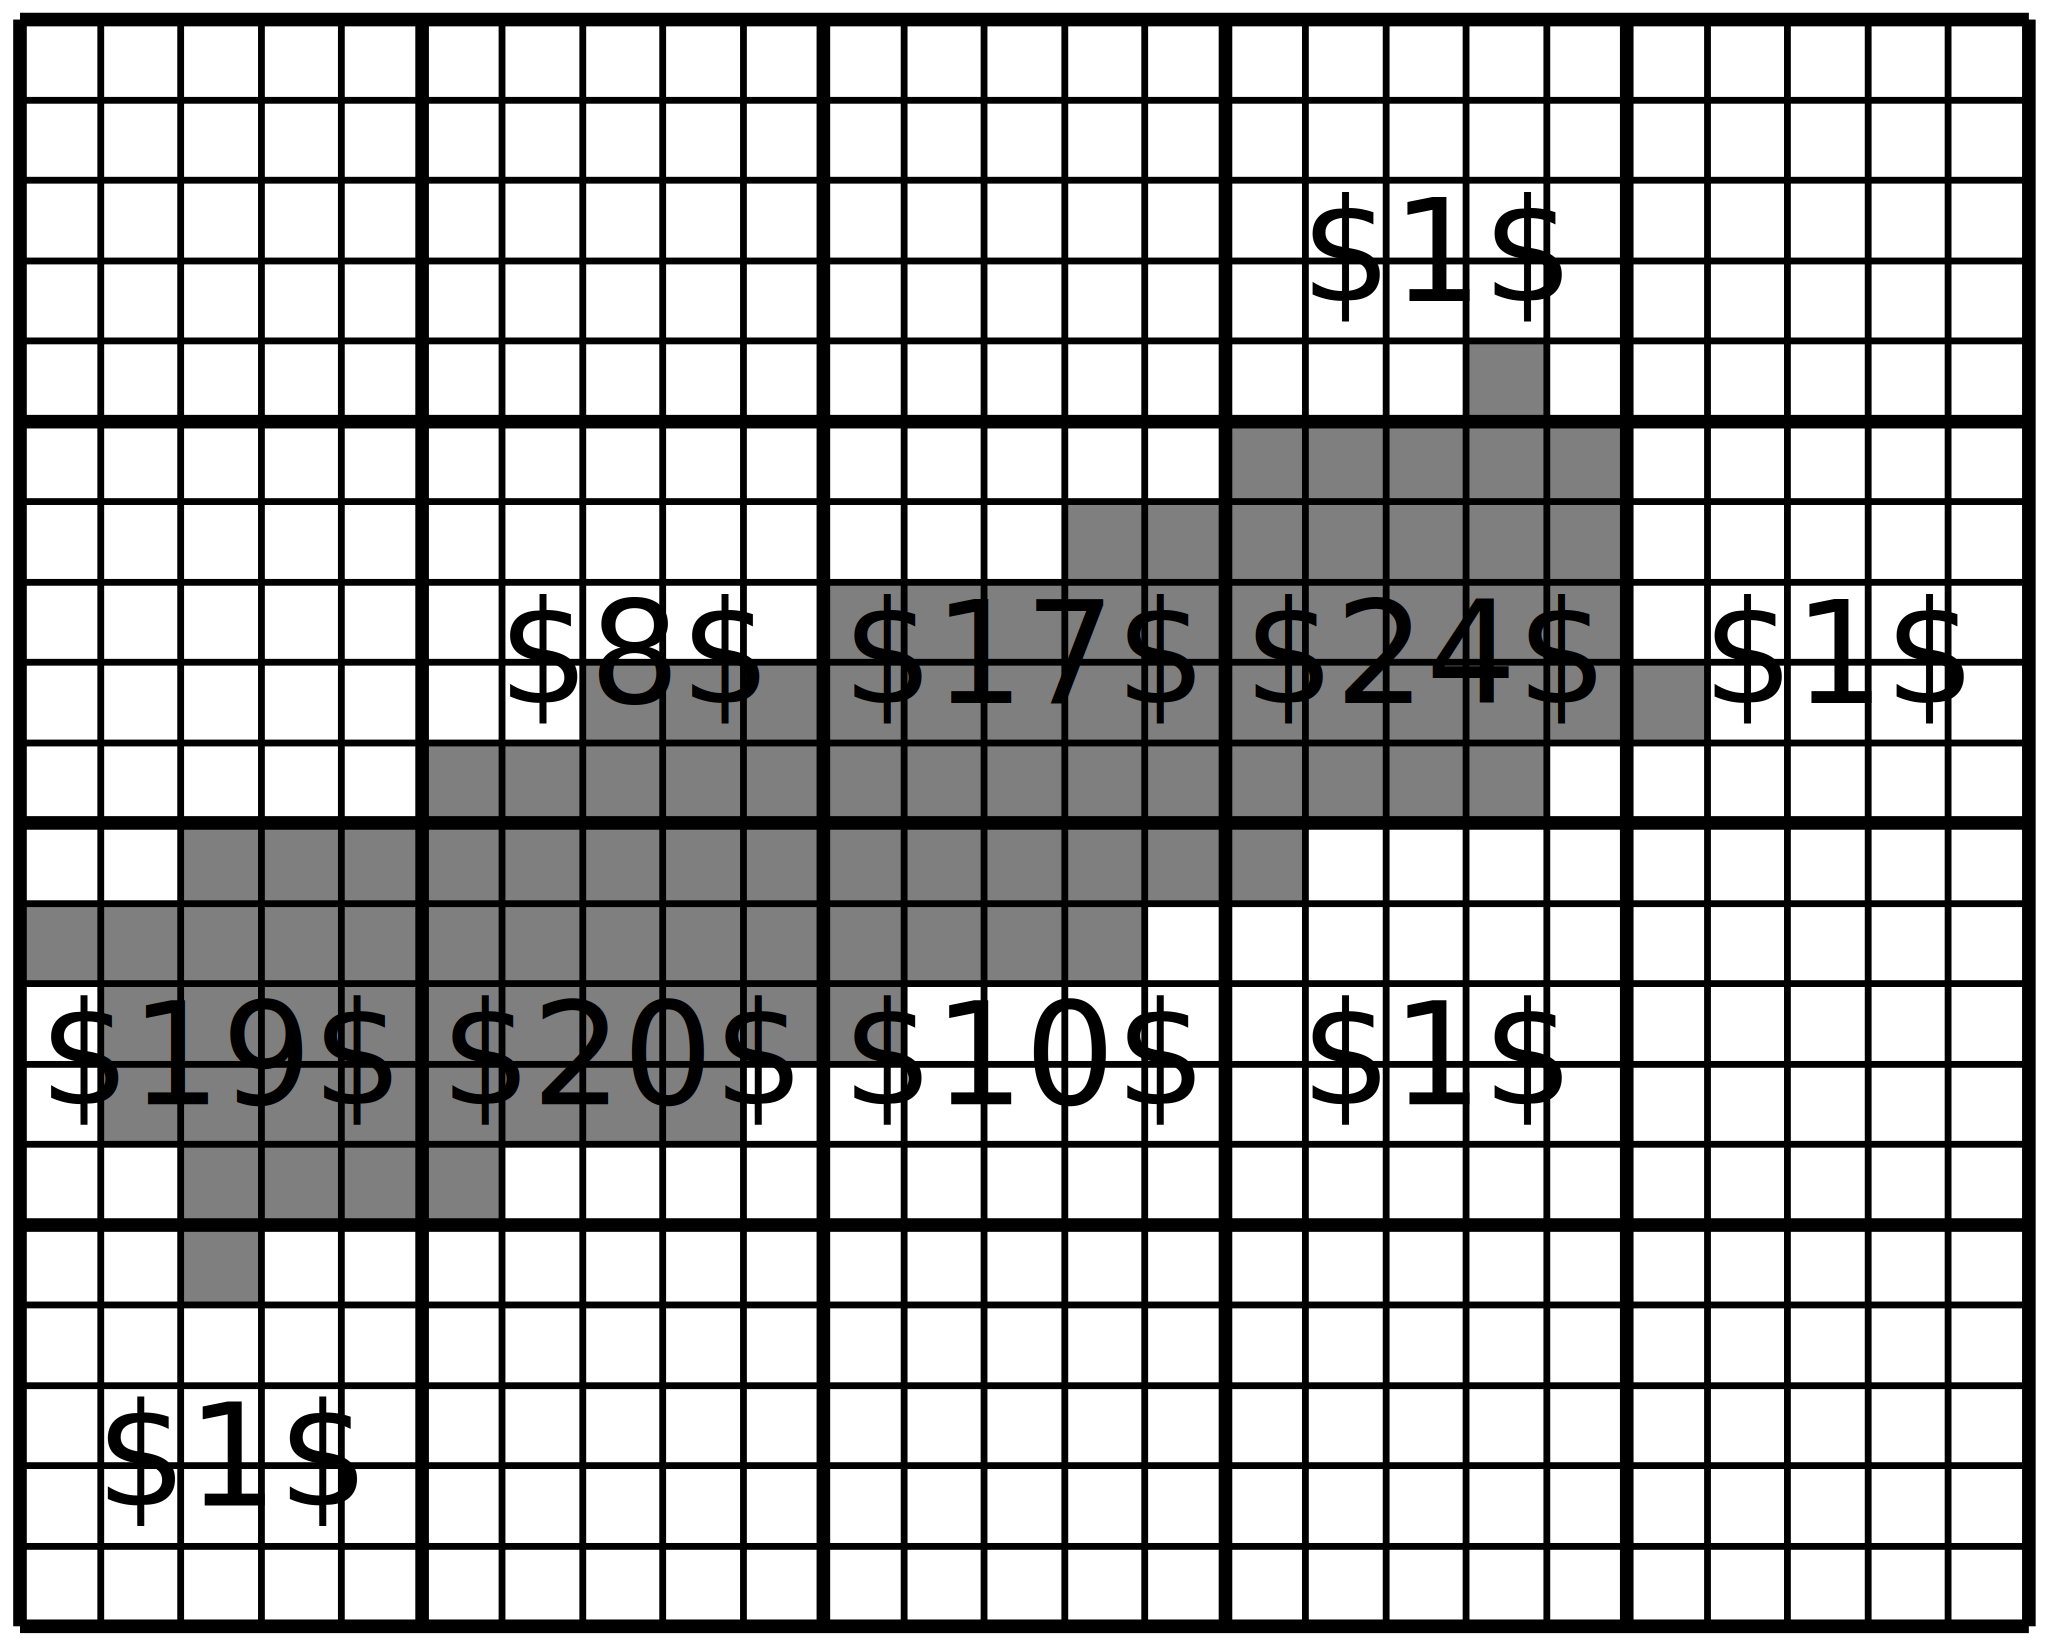
\includegraphics[width=\unitlength,page=1]{antial2.pdf}}%
    \put(0.49984237,0.45985708){\color[rgb]{0,0,0}\makebox(0,0)[b]{\smash{$17$}}}%
    \put(0.30706179,0.45985708){\color[rgb]{0,0,0}\makebox(0,0)[b]{\smash{$8$}}}%
    \put(0.69824506,0.45985708){\color[rgb]{0,0,0}\makebox(0,0)[b]{\smash{$24$}}}%
    \put(0.90269021,0.45985708){\color[rgb]{0,0,0}\makebox(0,0)[b]{\smash{$1$}}}%
    \put(0.10261665,0.26145439){\color[rgb]{0,0,0}\makebox(0,0)[b]{\smash{$19$}}}%
    \put(0.30101934,0.26145439){\color[rgb]{0,0,0}\makebox(0,0)[b]{\smash{$20$}}}%
    \put(0.49984237,0.26145439){\color[rgb]{0,0,0}\makebox(0,0)[b]{\smash{$10$}}}%
    \put(0.70386717,0.26145439){\color[rgb]{0,0,0}\makebox(0,0)[b]{\smash{$1$}}}%
    \put(0.10823876,0.0630517){\color[rgb]{0,0,0}\makebox(0,0)[b]{\smash{$1$}}}%
    \put(0.70386717,0.65868012){\color[rgb]{0,0,0}\makebox(0,0)[b]{\smash{$1$}}}%
  \end{picture}%
\endgroup%
 \raisebox{4.5em}{→} 
\includegraphics{antial3}
\end{center}

Verwenden Sie hierzu ein in beide Richtungen um einen Faktor $f$
verfeinertes Raster (in der Abbildung ist also $f = 5$). Fassen Sie die 
Linie in diesem feineren Raster als Rechteck auf und bestimmen Sie, 
welche (Sub-)Pixel eingefärbt werden müssen. Die Intensität der Pixel im
Originalraster wird dann proportional zur Anzahl der eingefärbten 
Subpixel gewählt.

Verwenden Sie bei der Programmierung \emph{kein} zusätzliches
zweidimensionales Feld; merken Sie sich statt dessen für jede
Subpixelzeile Anfangs- und Endpunkt des Rechtecks.

Testen Sie auch mit Linienbreiten $< 1$.
